\section{Results}

Total data usage across all operating systems and scenarios, aggregated for all tasks, is presented in Figure~\ref{fig-all-tasks-chart}. In all scenarios stock Android shows the highest data usage. Generally, configurations incorporating more Google services generate more traffic.

\begin{figure}
	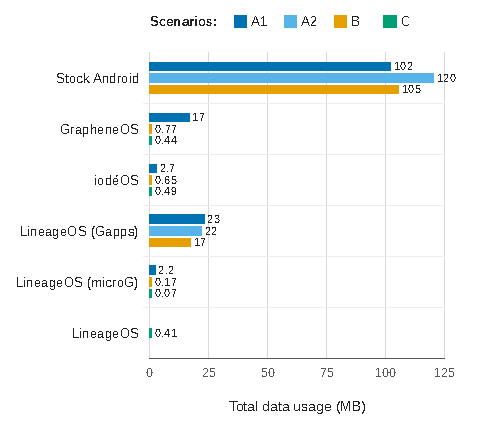
\includegraphics[width=\columnwidth]{images/all-tasks-data-usage-acm.pdf}
	\caption{Total data usage aggregated across all measurement tasks. Scenario applicability varies by system.} \label{fig-all-tasks-chart}
\end{figure}

\begin{figure}
	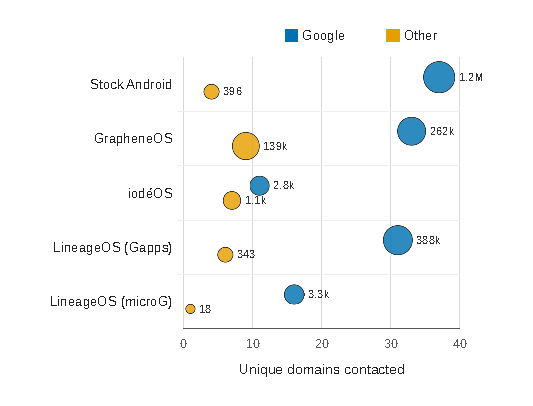
\includegraphics[width=\columnwidth]{images/os-domains-packets-acm.eps}
	\caption{Domains contacted in Scenario A1 aggregated for all tasks, grouped by operating system and by Google-related and other endpoints. Bubble size represents the total number of packets exchanged with each group. Vanilla LineageOS was omitted due to lack of available scenarios} \label{fig-domains-chart}
\end{figure}

Figure~\ref{fig-domains-chart} presents the domain-level distribution of network traffic. Stock Android contacts the most Google-related domains. iod\'eOS and LineageOS contact fewer servers overall. iod\'eOS also relies on some Mozilla infrastructure not present in other systems.

Table~\ref{tab:domains-mechanisms} shows the infrastructure dependencies for core system functions. LineageOS remains closest to stock Android, relying entirely on Google servers. iod\'eOS adopts an intermediate position, while GrapheneOS demonstrates the strongest de-Googling, substituting all three functions with its own or independently operated infrastructure.

Beyond aggregate traffic measurements, we were able to decrypt and analyze some payloads. A subset of these observations comes from earlier experiments performed on Android 14, because the Frida-based method was unsuccessful on Android 16.

Android's check-in mechanism transmits actual IMEI, MAC address, and hardware serial number to Google, while microG generates randomized, rotating identifiers (IMEI consistently prefixed with \texttt{35503104}, MAC addresses with OUI \texttt{b4:07:f9}). The Android ID field in microG requests is frequently empty or zeroed. The Google Advertising ID (ADID), formatted as a UUID, was observed in multiple requests on stock Android. This value remained constant across different requests, confirming its persistence as a cross-application tracking mechanism. After a manual reset in system settings, the ADID was transmitted as all zeros, indicating the identifier was actually cleared. We observed requests to \textit{app-measurement.com} on systems with Google services present, containing application package names, installation sources, versions, and the system theme preference.

When enabled, microG performs network geolocation without Google infrastructure by querying a selected provider, in our case \textit{api.position.xyz}. The request transmits nearby cell towers and returns approximate coordinates. We compared Google Play Store with Aurora Store (a popular application source in alternative Android distributions) by downloading the same application from each platform. Both stores retrieved identical packages from the same Google CDN infrastructure. However, the Play Store generated 106 requests, while Aurora Store produced 93.

In addition to network-level observations, Google Takeout\footnote{\url{https://takeout.google.com/}} was used to download data associated with test accounts for different Google services implementations. For every logged-in system, a corresponding entry appeared in \texttt{devices.json}, including device model, OS version, country, language, registration timestamp, and last activity time. However, the depth of telemetry varied considerably across configurations, as summarized in Table~\ref{tab:takeout-comparison}.

\begin{table}
	\caption{Domains observed for connectivity check, remote provisioning, and location assistance.}
	\label{tab:domains-mechanisms}
	
	\footnotesize
	\begin{tabular}{@{}p{0.11\columnwidth}p{0.3\columnwidth}p{0.25\columnwidth}p{0.22\columnwidth}@{}}
		\toprule
		System & Connectivity check& Provisioning & Location \\
		\midrule
		Stock & \url{connectivitycheck.gstatic.com} & -- & \url{supl.google.com}, \url{agnss.goog} \\
		Lineage & \url{connectivitycheck.gstatic.com} & \url{remoteprovisioning.googleapis.com} & \url{supl.google.com}, \url{agnss.goog} \\
		iod\'eOS & \url{captiveportal.kuketz.de} & \url{remoteprovisioning.googleapis.com} & \url{supl.google.com} \\
		Graphene & \url{connectivitycheck.grapheneos.network} & \url{remoteprovisioning.grapheneos.org} & \url{gs-loc.apple.grapheneos.org} \\
		\bottomrule
	\end{tabular}
\end{table}

\begin{table}
	\caption{Comparison of Google Takeout data across Android configurations.}
	\label{tab:takeout-comparison}

	\footnotesize
	\begin{tabular}{@{}p{0.25\columnwidth}p{0.23\columnwidth}p{0.20\columnwidth}p{0.20\columnwidth}@{}}
		\toprule
		System & Device IDs & Apps & Pixel telem. \\
		\midrule
		Stock Android & IMEI, serial & Extensive & Full \\
		Lineage (Gapps) & IMEI, serial & Extensive & Reduced \\
		Lineage (microG) & -- & -- & -- \\
		GrapheneOS & Falsified serial & 4 apps & -- \\
		\bottomrule
	\end{tabular}
\end{table}